\documentclass[]{presentation}
\usepackage{base}
\usepackage{draw}

\begin{document}

\begin{frame}
    \begin{figure}
        \centering
    \begin{tikzpicture}[scale=0.6]
        \draw[->, >=stealth] (-.5, .5) -- (11, .5);
        \draw[->, >=stealth] (0, -.5) -- (0, 8);
        \begin{scope}[xshift=-1cm]
        \foreach \x/\y/\n in {11/6/1, 5/7/2, 4/5/3, 5/1/4, 10/4/5, 10/1/6, 4/2/7, 2/2/8, 7/7/9}{
        \node[fill, minimum size=3pt, inner sep=0pt, circle] (\n) at (\x,\y) {};
        \draw(\n) node[above]{$x_{\n}$};
        }
        \end{scope}
        \end{tikzpicture}
     \end{figure}

    \begin{figure}
        \centering
    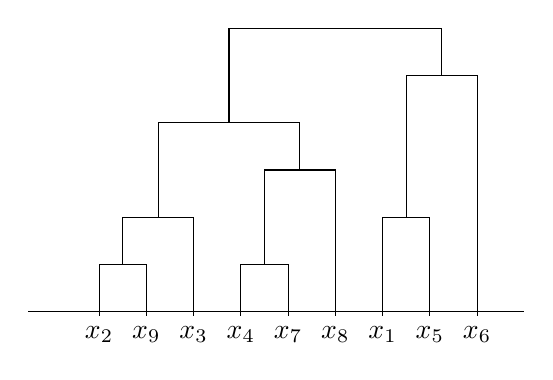
\begin{tikzpicture}[scale=0.6]
        \draw (-.5, 0) -- (10, 0);
        \foreach \x/\n in {1/2, 2/9, 3/3, 4/4, 5/7, 6/8, 7/1, 8/5, 9/6}
        \draw (\x, .1) -- (\x, -.1) node[below] {$x_{\n}$};
        
        \draw (1, 0) -- (1, 1) -- (2, 1) -- (2, 0);
        \draw (4, 0) -- (4, 1) -- (5, 1) -- (5, 0);
        \draw (4.5, 1) -- (4.5, 3) -- (6, 3) -- (6, 0);
        \draw (1.5, 1) -- (1.5, 2) -- (3, 2) -- (3, 0);
        \draw (7, 0) -- (7, 2) -- (8, 2) -- (8, 0);
        \draw (7.5, 2) -- (7.5, 5) -- (9, 5) -- (9, 0);
        \draw (2.25, 2) -- (2.25, 2*2) -- (5.25, 2*2) -- (5.25, 3);
        \draw (3.75, 2*2) -- (3.75, 6) -- (8.25, 6) -- (8.25, 5);
        \end{tikzpicture}
     \end{figure}
        
\end{frame}

\end{document}
